\documentclass[12pt]{article}

\title{Initial conditions}
\author{Jan Medlock et al.}

\usepackage{microtype}
\usepackage{tikz}
\usepackage{hyperref}
\hypersetup{breaklinks}
\hypersetup{pdfborder=0 0 0}
\usepackage{natbib}
\usepackage{hypernat}
\usepackage{amsmath}
\renewcommand{\vec}[1]{\mathbf{#1}}
\newcommand{\mat}[1]{\mathbf{#1}}
\DeclareMathOperator{\Prob}{Prob}
\DeclareMathOperator{\diag}{diag}
\newcommand{\md}{\mathrm{d}}
\newcommand{\me}{\mathrm{e}}
\newcommand{\mT}{\mathrm{T}}
\setcounter{MaxMatrixCols}{12}


\begin{document}

\maketitle

\section{Model}

We will find the equilibrium probability as a function of age of being
in each model compartment (\autoref{model_diagram}), i.e.
\begin{equation}
  P_X(a) = \Prob\{\text{in compartment $X$ at age $a$}|\text{alive at
    age $a$}\},
\end{equation}
for $X \in \{\mathrm{M}, \mathrm{S}, \mathrm{E}, \mathrm{I},
\mathrm{C}, \mathrm{R}, \mathrm{L}\}$
and $a \geq 0$.
We will assume that
\begin{itemize}
\item the infection hazard is constant,
\item all calves are born with maternal immunity, and
\item the hazard for antibody gain is constant.
\end{itemize}

\begin{figure}
  \begin{center}
    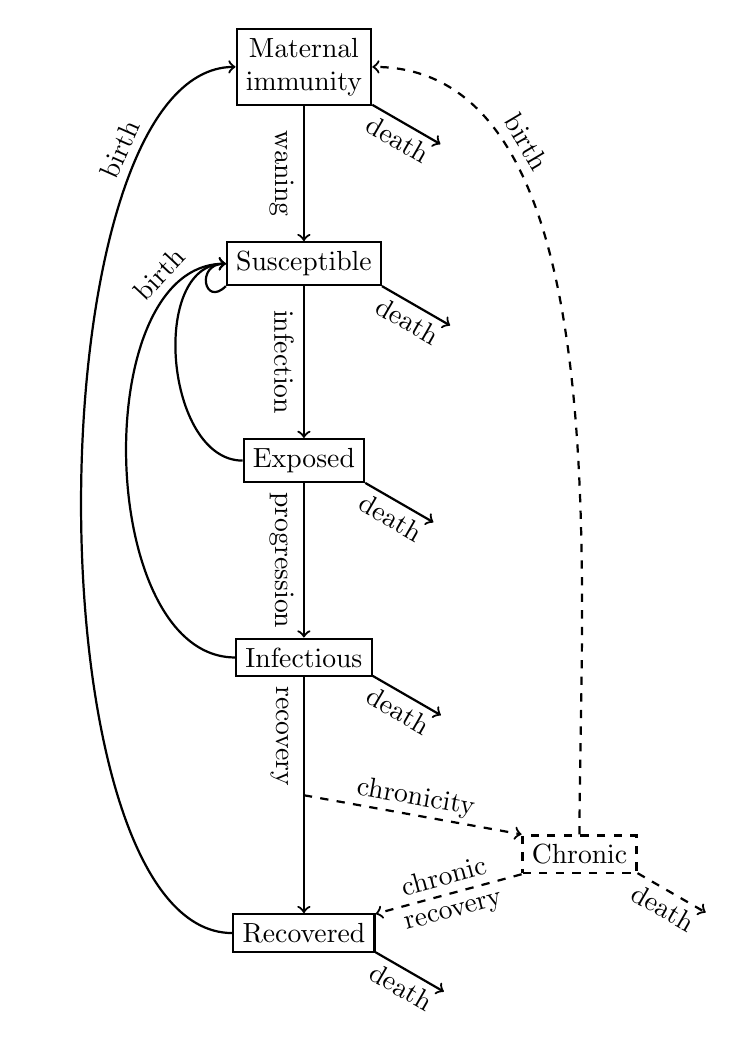
\begin{tikzpicture}[thick, compartment/.style = {rectangle, draw}]
  % Compartments.
  \node at (0, 11) [compartment, align=center, name=MaternalImmunity] {Maternal\\immunity};
  \node at (0, 8.5) [compartment, name=Susceptible] {Susceptible};
  \node at (0, 6) [compartment, name=Exposed] {Exposed};
  \node at (0, 3.5) [compartment, name=Infectious] {Infectious};
  \node at (0, 0) [compartment, name=Recovered] {Recovered};
  \node at (3.5, 1) [compartment, dashed, name=Chronic] {Chronic};

  % Location for branch from Infectious to Chronic and Recovered.
  \coordinate (recovery) at (0, 1.75);

  % Infection-related processes.
  \draw [->] (MaternalImmunity)
             to node [rotate=-90, below] {waning}
             (Susceptible);
  \draw [->] (Susceptible)
             to node [rotate=-90, below] {infection}
             (Exposed);
  \draw [->] (Exposed)
             to node [rotate=-90, below] {progression}
             (Infectious);
  \draw [  ] (Infectious)
             to node [rotate=-90, below, yshift=-2pt] {recovery}
             (recovery);
  \draw [->, dashed] (recovery)
             to node [sloped, above, yshift=-2pt] {chronicity}
             (Chronic.161);
  \draw [->] (recovery)
             to node [] {}
             (Recovered.90);
  \draw [->, dashed] (Chronic.199)
             to node [sloped, align=center] {chronic\\recovery}
             (Recovered.15);
  % \draw [->] (Recovered.195)
  %            to [out=180, in=180] node [left, align=center] {immunity\\waning}
  %            (Susceptible.180);

  % Births
  \draw [->] (Susceptible.196)
             to [out=225, in=180, looseness=3.5] node [] {}
             (Susceptible.180);
  \draw [->] (Exposed.180)
             to [out=180, in=180] node [] {}
             (Susceptible.180);
  \draw [->] (Infectious.180)
             to [out=180, in=180, looseness=0.9] node [sloped, above, pos=0.85] {birth}
             (Susceptible.180);
  \draw [->] (Recovered.180)
             to [out=180, in=180, looseness=0.6] node [sloped, above, pos=0.8] {birth}
             (MaternalImmunity.180);
  \draw [->, dashed] (Chronic.90)
             to [out=90, in=0, looseness=0.8] node [sloped, above, pos=0.75] {birth}
             (MaternalImmunity.0);

  % Deaths
  \draw [->] (MaternalImmunity.331)
             to node [sloped, below, yshift=1pt] {death}
             +(330: 1);
  \draw [->] (Susceptible.344)
             to node [sloped, below, yshift=1pt] {death}
             +(330: 1);
  \draw [->] (Exposed.340)
             to node [sloped, below, yshift=1pt] {death}
             +(330: 1);
  \draw [->] (Infectious.345)
             to node [sloped, below, yshift=1pt] {death}
             +(330: 1);
  \draw [->] (Recovered.345)
             to node [sloped, below, yshift=1pt] {death}
             +(330: 1);
  \draw [->, dashed] (Chronic.342)
             to node [sloped, below, yshift=1pt] {death}
             +(330: 1);
\end{tikzpicture}

%%% Local Variables:
%%% mode: latex
%%% TeX-master: "diagram_standalone"
%%% End:

  \end{center}
  \caption{Model diagram.}
  \label{model_diagram}
\end{figure}

\clearpage

For $a > 0$ and $0 < r \leq a$,
the compartment probabilities satisfy
\begin{align}
  P_{\mathrm{M}}(0) &= 1,
  \\
  \frac{\md P_{\mathrm{M}}}{\md a}
  &= - h_{\text{waning}}(a) P_{\mathrm{M}}(a),
  \displaybreak[0]\\
  P_{\mathrm{S}}(0) &= 0,
  \\
  \frac{\md P_{\mathrm{S}}}{\md a}
  &= h_{\text{waning}}(a) P_{\mathrm{M}}(a)
  - h_{\text{infection}} P_{\mathrm{S}}(a),
  \displaybreak[0]\\
  p_{\mathrm{E}}(0, 0) &= 0,
  \\
  p_{\mathrm{E}}(a, 0) &= h_{\text{infection}}
  \left[P_{\mathrm{S}}(a) + P_{\mathrm{L}}(a)\right],
  \\
  \left(\frac{\partial}{\partial a}
    + \frac{\partial}{\partial r}\right)
  p_{\mathrm{E}}
  &= - h_{\text{progression}}(r) p_{\mathrm{E}}(a, r),
  \displaybreak[0]\\
  p_{\mathrm{I}}(0, 0) &= 0,
  \\
  p_{\mathrm{I}}(a, 0) &=
  \int_0^a h_{\text{progression}}(r)
  p_{\mathrm{E}}(a, r) \md r,
  \\
  \left(\frac{\partial}{\partial a}
    + \frac{\partial}{\partial r}\right)
  p_{\mathrm{I}}
  &= - h_{\text{recovery}}(r) p_{\mathrm{I}}(a, r),
  \displaybreak[0]\\
  p_{\mathrm{C}}(0, 0) &= 0,
  \\
  p_{\mathrm{C}}(a, 0)
  &= p_{\text{chronicity}}
  \int_0^a h_{\text{recovery}}(r) p_{\mathrm{I}}(a, r) \md r,
  \\
  \left(\frac{\partial}{\partial a}
    + \frac{\partial}{\partial r}\right)
  p_{\mathrm{C}}
  &= - h_{\text{chronic recovery}}(r) p_{\mathrm{C}}(a, r),
  \displaybreak[0]\\
  P_{\mathrm{R}}(0) &= 0,
  \\
  \begin{split}
    \frac{\md P_{\mathrm{R}}}{\md a} &=
    \left(1 - p_{\text{chronicity}}\right)
    \int_0^a h_{\text{recovery}}(r) p_{\mathrm{I}}(a, r) \md r
    \\ & \quad {}
    + \int_0^a h_{\text{chronic recovery}}(r) p_{\mathrm{C}}(a, r) \md r
    \\ & \quad {}
    + h_{\text{antibody gain}} P_{\mathrm{L}}(a)
    - h_{\text{antibody loss}} P_{\mathrm{R}}(a),
  \end{split}
  \displaybreak[0]\\
  P_{\mathrm{L}}(0) &= 0,
  \\
  \frac{\md P_{\mathrm{L}}}{\md a} &=
  h_{\text{antibody loss}} P_{\mathrm{R}}(a)
  - \left(h_{\text{antibody gain}} + h_{\text{infection}}\right)
  P_{\mathrm{L}}(a).
\end{align}


\subsection{Analysis}

Integrating the PDEs along the characteristics $r = a - a_0$ gives
\begin{align}
  P_{\mathrm{M}}(0) &= 1,
  \\
  \frac{\md P_{\mathrm{M}}}{\md a}
  &= - h_{\text{waning}}(a) P_{\mathrm{M}}(a),
  \displaybreak[0]\\
  P_{\mathrm{S}}(0) &= 0,
  \\
  \frac{\md P_{\mathrm{S}}}{\md a}
  &= h_{\text{waning}}(a) P_{\mathrm{M}}(a)
  - h_{\text{infection}} P_{\mathrm{S}}(a),
  \displaybreak[0]\\
  p_{\mathrm{E}}(0, 0) &= 0,
  \\
  p_{\mathrm{E}}(a, 0) &= h_{\text{infection}}
  \left[P_{\mathrm{S}}(a) + P_{\mathrm{L}}(a)\right],
  \\
  p_{\mathrm{E}}(a, r)
  &= S_{\text{progression}}(r) p_{\mathrm{E}}(a - r, 0),
  \displaybreak[0]\\
  p_{\mathrm{I}}(0, 0) &= 0,
  \\
  p_{\mathrm{I}}(a, 0)
  &= \int_0^a p_{\text{progression}}(r)
  p_{\mathrm{E}}(a - r, 0) \md r,
  \\
  p_{\mathrm{I}}(a, r)
  &= S_{\text{recovery}}(r) p_{\mathrm{I}}(a - r, 0),
  \displaybreak[0]\\
  p_{\mathrm{C}}(0, 0) &= 0,
  \\
  p_{\mathrm{C}}(a, 0)
  &= p_{\text{chronicity}}
  \int_0^a p_{\text{recovery}}(r) p_{\mathrm{I}}(a - r, 0) \md r,
  \\
  p_{\mathrm{C}}(a, r)
  &= S_{\text{chronic recovery}}(r) p_{\mathrm{C}}(a - r, 0),
  \displaybreak[0]\\
  P_{\mathrm{R}}(0) &= 0,
  \\
  \begin{split}
    \frac{\md P_{\mathrm{R}}}{\md a} &=
    \left(1 - p_{\text{chronicity}}\right)
    \int_0^a p_{\text{recovery}}(r) p_{\mathrm{I}}(a - r, 0) \md r
    \\ & \quad {}
    + \int_0^a p_{\text{chronic recovery}}(r) p_{\mathrm{C}}(a - r, 0) \md r
    \\ & \quad {}
    + h_{\text{antibody gain}} P_{\mathrm{L}}(a)
    - h_{\text{antibody loss}} P_{\mathrm{R}}(a),
  \end{split}
  \displaybreak[0]\\
  P_{\mathrm{L}}(0) &= 0,
  \\
  \frac{\md P_{\mathrm{L}}}{\md a} &=
  h_{\text{antibody loss}} P_{\mathrm{R}}(a)
  - \left(h_{\text{antibody gain}} + h_{\text{infection}}\right)
  P_{\mathrm{L}}(a).
\end{align}

Let
\begin{equation}
  P(a) = P_{\mathrm{M}}(a) + P_{\mathrm{S}}(a)
  + P_{\mathrm{E}}(a) + P_{\mathrm{I}}(a)
  + P_{\mathrm{C}}(a) + P_{\mathrm{R}}(a)
  + P_{\mathrm{L}}(a),
\end{equation}
with
\begin{align}
  \begin{split}
    P_{\mathrm{E}}(a) &= \int_0^a p_{\mathrm{E}}(a, r) \md r
    \\
    &= \int_0^a S_{\text{progression}}(a - a_0) p_{\mathrm{E}}(a_0, 0) \md a_0,
  \end{split}
  \displaybreak[0]\\
  \begin{split}
    P_{\mathrm{I}}(a) &= \int_0^a p_{\mathrm{I}}(a, r) \md r
    \\
    &= \int_0^a S_{\text{recovery}}(a - a_0) p_{\mathrm{I}}(a_0, 0) \md a_0,
  \end{split}
  \displaybreak[0]\\
  \begin{split}
    P_{\mathrm{C}}(a) &= \int_0^a p_{\mathrm{C}}(a, r) \md r
    \\
    &= \int_0^a S_{\text{chronic recovery}}(a - a_0) p_{\mathrm{C}}(a_0, 0) \md a_0,
  \end{split}
\end{align}
so that
\begin{align}
  \begin{split}
    \frac{\md P_{\mathrm{E}}}{\md a}
    &= \frac{\md}{\md a}
    \int_0^a S_{\text{progression}}(a - a_0) p_{\mathrm{E}}(a_0, 0) \md a_0
    \\
    &= p_{\mathrm{E}}(a, 0)
    -
    \int_0^a p_{\text{progression}}(a - a_0) p_{\mathrm{E}}(a_0, 0) \md a_0
    \\
    &= h_{\text{infection}}
    \left[P_{\mathrm{S}}(a) + P_{\mathrm{L}}(a)\right]
    - \int_0^a p_{\text{progression}}(r) p_{\mathrm{E}}(a - r, 0) \md r,
  \end{split}
  \displaybreak[0]\\
  \begin{split}
    \frac{\md P_{\mathrm{I}}}{\md a}
    &= \frac{\md}{\md a}
    \int_0^a S_{\text{recovery}}(a - a_0) p_{\mathrm{I}}(a_0, 0) \md a_0
    \\
    &= p_{\mathrm{I}}(a, 0)
    -
    \int_0^a p_{\text{recovery}}(a - a_0) p_{\mathrm{I}}(a_0, 0) \md a_0
    \\
    &= \int_0^a p_{\text{progression}}(r) p_{\mathrm{E}}(a - r, 0) \md r
    - \int_0^a p_{\text{recovery}}(r) p_{\mathrm{I}}(a - r, 0) \md r,
  \end{split}
  \displaybreak[0]\\
  \begin{split}
    \frac{\md P_{\mathrm{C}}}{\md a}
    &= \frac{\md}{\md a}
    \int_0^a S_{\text{chronic recovery}}(a - a_0) p_{\mathrm{C}}(a_0, 0) \md a_0
    \\
    &= p_{\mathrm{C}}(a, 0)
    -
    \int_0^a p_{\text{chronic recovery}}(a - a_0) p_{\mathrm{C}}(a_0, 0) \md a_0
    \\
    &= p_{\text{chronicity}}
    \int_0^a p_{\text{recovery}}(r) p_{\mathrm{I}}(a - r, 0) \md r
    \\ & \quad {}
    - \int_0^a p_{\text{chronic recovery}}(r) p_{\mathrm{C}}(a - r, 0) \md r,
  \end{split}
\end{align}
and then
\begin{equation}
  \frac{\md P}{\md a} =
  \frac{\md P_{\mathrm{M}}}{\md a}
  + \frac{\md P_{\mathrm{S}}}{\md a}
  + \frac{\md P_{\mathrm{E}}}{\md a}
  + \frac{\md P_{\mathrm{I}}}{\md a}
  + \frac{\md P_{\mathrm{C}}}{\md a}
  + \frac{\md P_{\mathrm{R}}}{\md a}
  + \frac{\md P_{\mathrm{L}}}{\md a}
  = 0.
\end{equation}


\section{Numerical method}

To compute the compartment probabilities, we used the Crank--Nicolson
method on characteristics and the composite trapezoid rule for the
integrals \citep{milner_1992}.  Given the age step $\Delta a$,
for $i \in \{0, 1, 2, \ldots, I - 1\}$ and
$j \in \{0, 1, 2, \ldots, i\}$, let $a^i = i \Delta a$,
$P_X^i \approx P_X(a^i)$, and
$p_X^i \approx p_X(a^i, 0)$.
For each $i \in \{1, 2, \ldots, I - 1\}$, using the
Crank--Nicolson method on characteristics and,
for $Y \in \{\text{progression}, \text{recovery},
\text{chronic recovery}\}$,
\begin{equation}
  p_Y(r^j) = - \frac{\md S_Y}{\md r} (r^j)
  \approx \frac{S_Y(r^{j - 1}) - S_Y(r^j)}{\Delta a},
\end{equation}
gives
\begin{align}
  P_{\mathrm{M}}^0 &= 1,
  \\
  \frac{P_{\mathrm{M}}^i - P_{\mathrm{M}}^{i - 1}}{\Delta a}
  &= - h_{\text{waning}}(a^{i - 1 / 2})
  \frac{P_{\mathrm{M}}^i + P_{\mathrm{M}}^{i - 1}}{2},
  \displaybreak[0]\\
  P_{\mathrm{S}}^0 &= 0,
  \\
  \frac{P_{\mathrm{S}}^i - P_{\mathrm{S}}^{i - 1}}{\Delta a}
  &= h_{\text{waning}}(a^{i - 1 / 2})
  \frac{P_{\mathrm{M}}^i + P_{\mathrm{M}}^{i - 1}}{2}
  - h_{\text{infection}}
  \frac{P_{\mathrm{S}}^i + P_{\mathrm{S}}^{i - 1}}{2},
  \displaybreak[0]\\
  p_{\mathrm{E}}^0 &= 0,
  \\
  p_{\mathrm{E}}^i &= h_{\text{infection}}
  \left(\frac{P_{\mathrm{S}}^i + P_{\mathrm{S}}^{i - 1}}{2}
        + \frac{P_{\mathrm{L}}^i + P_{\mathrm{L}}^{i - 1}}{2}\right)
  \displaybreak[0]\\
  p_{\mathrm{I}}^0 &= 0,
  \\
  p_{\mathrm{I}}^i
  &= \sum_{j = 1}^i \left[S_{\text{progression}}(r^{j - 1})
    - S_{\text{progression}}(r^j)\right]
  p_{\mathrm{E}}^{i - j},
  \displaybreak[0]\\
  p_{\mathrm{C}}^0 &= 0,
  \\
  p_{\mathrm{C}}^i
  &= p_{\text{chronicity}}
  \sum_{j = 1}^i \left[S_{\text{recovery}}(r^{j - 1})
    - S_{\text{recovery}}(r^j)\right]
  p_{\mathrm{I}}^{i - j},
  \displaybreak[0]\\
  P_{\mathrm{R}}^0 &= 0,
  \\
  \begin{split}
    \frac{P_{\mathrm{R}}^i - P_{\mathrm{R}}^{i - 1}}{\Delta a}
    &= \left(1 - p_{\text{chronicity}}\right)
    \sum_{j = 1}^i \left[S_{\text{recovery}}(r^{j - 1})
      - S_{\text{recovery}}(r^j)\right]
    p_{\mathrm{I}}^{i - j}
    \\ & \quad {}
    + \sum_{j = 1}^i \left[S_{\text{chronic recovery}}(r^{j - 1})
      - S_{\text{chronic recovery}}(r^j)\right]
    p_{\mathrm{C}}^{i - j}
    \\ & \quad {}
    + h_{\text{antibody gain}}
    \frac{P_{\mathrm{L}}^i + P_{\mathrm{L}}^{i - 1}}{2}
    - h_{\text{antibody loss}}
    \frac{P_{\mathrm{R}}^i + P_{\mathrm{R}}^{i - 1}}{2},
  \end{split}
  \displaybreak[0]\\
  P_{\mathrm{L}}^0 &= 0,
  \\
  \begin{split}
    \frac{P_{\mathrm{L}}^i - P_{\mathrm{L}}^{i - 1}}{\Delta a}
    &= h_{\text{antibody loss}}
    \frac{P_{\mathrm{R}}^i + P_{\mathrm{R}}^{i - 1}}{2}
    \\ & \quad {}
    - \left(h_{\text{antibody gain}} + h_{\text{infection}}\right)
    \frac{P_{\mathrm{L}}^i + P_{\mathrm{L}}^{i - 1}}{2}.
  \end{split}
\end{align}
That is,
\begin{align}
  P_{\mathrm{M}}^0 &= 1,
  \\
  - \left[1 - \frac{h_{\text{waning}}(a^{i - 1 / 2}) \Delta a}{2}\right]
  P_{\mathrm{M}}^{i - 1}
  + \left[1 + \frac{h_{\text{waning}}(a^{i - 1 / 2}) \Delta a}{2}\right]
  P_{\mathrm{M}}^i
  &= 0,
  \displaybreak[0]\\
  P_{\mathrm{S}}^0 &= 0,
  \\
  \begin{split}
    - \frac{h_{\text{waning}}(a^{i - 1 / 2}) \Delta a}{2}
    P_{\mathrm{M}}^{i - 1}
    - \frac{h_{\text{waning}}(a^{i - 1 / 2}) \Delta a}{2}
    P_{\mathrm{M}}^i
    \\ {}
    - \left[1 - \frac{h_{\text{infection}} \Delta a}{2}\right]
    P_{\mathrm{S}}^{i - 1}
    + \left[1 + \frac{h_{\text{infection}} \Delta a}{2}\right]
    P_{\mathrm{S}}^i
    &= 0,
  \end{split}
  \displaybreak[0]\\
  p_{\mathrm{E}}^0 &= 0,
  \\
  \begin{split}
    - \frac{h_{\text{infection}}}{2} P_{\mathrm{S}}^{i - 1}
    - \frac{h_{\text{infection}}}{2} P_{\mathrm{S}}^i
    \\ {}
    + p_{\mathrm{E}}^i
    \\ {}
    - \frac{h_{\text{infection}}}{2} P_{\mathrm{L}}^{i - 1}
    - \frac{h_{\text{infection}}}{2} P_{\mathrm{L}}^i
    &= 0,
  \end{split}
  \displaybreak[0]\\
  p_{\mathrm{I}}^0 &= 0,
  \\
  - \sum_{j = 1}^i
  \left[S_{\text{progression}}(r^{j - 1})
  - S_{\text{progression}}(r^j)\right]
  p_{\mathrm{E}}^{i - j}
  + p_{\mathrm{I}}^i
  &= 0,
  \displaybreak[0]\\
  p_{\mathrm{C}}^0 &= 0,
  \\
  - \sum_{j = 1}^i
  p_{\text{chronicity}} \left[S_{\text{recovery}}(r^{j - 1})
  - S_{\text{recovery}}(r^j)\right]
  p_{\mathrm{I}}^{i - j}
  + p_{\mathrm{C}}^i
  &= 0,
  \displaybreak[0]\\
  P_{\mathrm{R}}^0 &= 0,
  \\
  \begin{split}
    - \sum_{j = 1}^i
    \left(1 - p_{\text{chronicity}}\right)
    \left[S_{\text{recovery}}(r^{j - 1})
      - S_{\text{recovery}}(r^j)\right] \Delta a
    p_{\mathrm{I}}^{i - j}
    \\ {}
    - \sum_{j = 1}^i
    \left[S_{\text{chronic recovery}}(r^{j - 1})
      - S_{\text{chronic recovery}}(r^j)\right] \Delta a
    p_{\mathrm{C}}^{i - j}
    \\ {}
    - \left[1 - \frac{h_{\text{antibody loss}} \Delta a}{2}\right]
    P_{\mathrm{R}}^{i - 1}
    + \left[1 + \frac{h_{\text{antibody loss}} \Delta a}{2}\right]
    P_{\mathrm{R}}^i
    \\ {}
    - \frac{h_{\text{antibody gain}} \Delta a}{2}
    P_{\mathrm{L}}^{i - 1}
    - \frac{h_{\text{antibody gain}} \Delta a}{2}
    P_{\mathrm{L}}^i
    &= 0,
  \end{split}
  \displaybreak[0]\\
  P_{\mathrm{L}}^0 &= 0,
  \\
  \begin{split}
    - \frac{h_{\text{antibody loss}} \Delta a}{2}
    P_{\mathrm{R}}^{i - 1}
    - \frac{h_{\text{antibody loss}} \Delta a}{2}
    P_{\mathrm{R}}^i
    \\ {}
    - \left[1
      - \frac{(h_{\text{antibody gain}} + h_{\text{infection}}) \Delta a}{2}\right]
    P_{\mathrm{L}}^{i - 1}
    \\ {}
    + \left[1
      + \frac{(h_{\text{antibody gain}} + h_{\text{infection}}) \Delta a}{2}\right]
    P_{\mathrm{L}}^i
    &= 0.
  \end{split}
\end{align}
The coefficients must be non-negative to ensure each component of the
$P_X$'s and $p_X$'s is non-negative. In particular, the hazards must
satisfy
\begin{equation}
  2 - h \Delta a \geq 0,
\end{equation}
or
\begin{equation}
  h \leq \frac{2}{\Delta a}.
\end{equation}


\subsection{Analysis}

The integrals of the PDE variables over $r$ satisfy
\begin{align}
  P_{\mathrm{E}}^i
  &= \sum_{j = 0}^i S_{\text{progression}}(r^j) p_{\mathrm{E}}^{i - j} \Delta a,
  \displaybreak[0]\\
  P_{\mathrm{I}}^i
  &= \sum_{j = 0}^i S_{\text{recovery}}(r^j) p_{\mathrm{I}}^{i - j} \Delta a,
  \displaybreak[0]\\
  P_{\mathrm{C}}^i
  &= \sum_{j = 0}^i S_{\text{chronic recovery}}(r^j) p_{\mathrm{C}}^{i - j} \Delta a,
\end{align}
so that
\begin{align}
  \begin{split}
    \frac{P_{\mathrm{E}}^i - P_{\mathrm{E}}^{i - 1}}{\Delta a}
    &= \sum_{j = 0}^i S_{\text{progression}}(r^j) p_{\mathrm{E}}^{i - j}
    - \sum_{j = 0}^{i - 1} S_{\text{progression}}(r^j) p_{\mathrm{E}}^{i - 1 - j}
    \\
    &= p_{\mathrm{E}}^i
    - \sum_{j = 1}^i \left[S_{\text{progression}}(r^{j - 1})
      - S_{\text{progression}}(r^j)\right]
    p_{\mathrm{E}}^{i - j}
    \\
    &= h_{\text{infection}}
    \left(\frac{P_{\mathrm{S}}^i + P_{\mathrm{S}}^{i - 1}}{2}
        + \frac{P_{\mathrm{L}}^i + P_{\mathrm{L}}^{i - 1}}{2}\right)
    \\ & \quad {}
    - \sum_{j = 1}^i \left[S_{\text{progression}}(r^{j - 1})
      - S_{\text{progression}}(r^j)\right]
    p_{\mathrm{E}}^{i - j},
  \end{split}
  \displaybreak[0]\\
  \begin{split}
    \frac{P_{\mathrm{I}}^i - P_{\mathrm{I}}^{i - 1}}{\Delta a}
    &= \sum_{j = 0}^i S_{\text{recovery}}(r^j) p_{\mathrm{I}}^{i - j}
    - \sum_{j = 0}^{i - 1} S_{\text{recovery}}(r^j) p_{\mathrm{I}}^{i - 1 - j}
    \\
    &= p_{\mathrm{I}}^i
    - \sum_{j = 1}^i \left[S_{\text{recovery}}(r^{j - 1})
      - S_{\text{recovery}}(r^j)\right]
    p_{\mathrm{I}}^{i - j}
    \\
    &= \sum_{j = 1}^i \left[S_{\text{progression}}(r^{j - 1})
      - S_{\text{progression}}(r^j)\right]
    p_{\mathrm{E}}^{i - j}
    \\ & \quad {}
    - \sum_{j = 1}^i \left[S_{\text{recovery}}(r^{j - 1})
      - S_{\text{recovery}}(r^j)\right]
    p_{\mathrm{I}}^{i - j},
  \end{split}
  \displaybreak[0]\\
  \begin{split}
    \frac{P_{\mathrm{C}}^i - P_{\mathrm{C}}^{i - 1}}{\Delta a}
    &= \sum_{j = 0}^i S_{\text{chronic recovery}}(r^j) p_{\mathrm{C}}^{i - j}
    - \sum_{j = 0}^{i - 1} S_{\text{chronic recovery}}(r^j) p_{\mathrm{C}}^{i - 1 - j}
    \\
    &= p_{\mathrm{C}}^i
    - \sum_{j = 1}^i \left[S_{\text{chronic recovery}}(r^{j - 1})
      - S_{\text{chronic recovery}}(r^j)\right]
    p_{\mathrm{C}}^{i - j}
    \\
    &= p_{\text{chronicity}}
    \sum_{j = 1}^i \left[S_{\text{recovery}}(r^{j - 1})
      - S_{\text{recovery}}(r^j)\right] p_{\mathrm{I}}^{i - j}
    \\ & \quad {}
    - \sum_{j = 1}^i \left[S_{\text{chronic recovery}}(r^{j - 1})
      - S_{\text{chronic recovery}}(r^j)\right]
    p_{\mathrm{C}}^{i - j}.
  \end{split}
\end{align}
Then, for
\begin{equation}
  P^i = P_{\mathrm{M}}^i + P_{\mathrm{S}}^i + P_{\mathrm{E}}^i
  + P_{\mathrm{I}}^i + P_{\mathrm{C}}^i + P_{\mathrm{R}}^i
  + P_{\mathrm{L}}^i,
\end{equation}
we have
\begin{align}
  P^0 &= 1,
  \\
  \frac{P^i - P^{i - 1}}{\Delta a} &= 0,
\end{align}
so that
\begin{equation}
  P^i = 1,
\end{equation}
for all $i \in \{1, 2, \ldots, I - 1\}$.


\bibliography{journal_abbreviations,math_epi}
\bibliographystyle{jpmbib}

\end{document}
